\documentclass[a4paper,12pt]{article}
\usepackage[ukrainian,english]{babel}
\usepackage{ucs}
\usepackage[utf8]{inputenc}
\usepackage[T2A]{fontenc}
\usepackage{amsmath}
\usepackage{amsfonts}
\usepackage{graphicx}
\usepackage{changepage}
\usepackage{multirow}
\usepackage{subcaption}
\usepackage{array, makecell}
\usepackage[document]{ragged2e}
\usepackage{parskip}
\usepackage[paper=portrait,pagesize]{typearea}
\usepackage{multicol}
\newcommand\tab[1][1cm]{\hspace*{#1}}
\addto\captionsenglish{\renewcommand{\figurename}{Рис.}}
\addto\captionsenglish{\renewcommand{\tablename}{Таблиця}}
\captionsetup[table]{justification=raggedleft,singlelinecheck=off}
\usepackage{titlesec}
\usepackage[left=20mm, top=20mm, right=20mm, bottom=20mm, nohead, nofoot]{geometry}
\titleformat{\section}[block]{\Large\bfseries\filcenter}{}{1em}{}
\titleformat{\subsection}[hang]{\bfseries}{}{1em}{}
\titleformat{\subsubsection}[hang]{\bfseries}{}{2em}{}
\begin{document}
	\begin{justify}
		\thispagestyle{empty}\setlength{\parindent}{0pt}
	\begin{center}
		\textbf{НАЦІОНАЛЬНИЙ ТЕХНІЧНИЙ УНІВЕРСИТЕТ УКРАЇНИ}\\ 
		\textbf{«КИЇВСЬКИЙ ПОЛІТЕХНІЧНИЙ ІНСТИТУТ»}\\ 
		\textbf{ФІЗИКО-ТЕХНІЧНИЙ ІНСТИТУТ}
	\end{center}
	$\\\\\\\\\\\\\\\\\\\\\\\\\\$
	\begin{center}
		Лабораторна робота з фізики №1\bigbreak
ЕЛЕКТРИЧНІ ПОЛЯ ТА ПОТЕНЦІАЛИ ЗАРЯДЖЕНИХ ТІЛ 
	\end{center}
	$\\\\\\\\\\\\\\\\\\\\\\\\\\$
	\begin{flushright}
	Виконалa:\\
		студент групи ФІ-12\\
		Бекешева Анастасія 
	\end{flushright}
	$\\\\\\\\\\$
	\begin{center}
		\textbf{Київ-2022}
	\end{center}
	\newpage
	\begin{center}
		\section* {РОЗДІЛ 1. Теоретична довiдка.}
	\end{center}
	\textbf{Ключові поняття:} Електричне поле, електричний заряд, напруженість поля, електростатичний потенціал, потік вектора напруженості поля, електрична індукція, поверхнева густина заряду, поляризація, діелектрична стала, теорема Гауса, метод електричних зображень.\newline\\
		\textbf{Мета роботи: }Встановити залежність електричного потенціалу зарядженої кулі від відстані від центру кулі та напруженість поля, яке виникає при цьому.
		\subsection{Теоретичне підгрунтя: }
	З закону Кулона, поле точкового електричного заряду $q$ задається виразом:
	$$\vec{E}=\dfrac{kq}{r^2} \eqno(1)$$
	
	В деяких випадках для розрахунку електричного поля довільної конфігурації зарядів можна скористатись теоремою Гауса в диференціальному вигляді:
	$$div\vec{E}=\dfrac{\rho}{\varepsilon} \eqno(2)$$
	
	Для розрахунку електричного поля, що утворюється довільною системою зарядів теореми Гауса недостатньо. Це видно з того, що співвідношення (2) скалярне, а $\vec{E}$ векторна величина.
	
	Можна показати, що електричне поле є потенційне поле, тобто робота по переміщенню точкового заряда з точки 1 в точку 2 в електростатичному полі не залежить від форми шляху переходу. Корисно ввести поняття різниці потенціалів $\varphi_1-\varphi_2$ як роботи по переміщенню одиниці заряду в електричному полі:
	$$A_{1 2}=q(\varphi_1-\varphi_2) \eqno(3)$$
	
	Користуючись цим визначенням, а також визначенням напруженості електричного поля легко встановити зв'язок між потенціалом та електричним полем:
	$$\vec{E}=-grad\varphi \eqno(4)$$
	
	Якщо відомий потенціал $\varphi(x,\: y,\: z)$, то напруженість електричного поля можна розрахувати, диференціюючи потенціал по координатах, і навпаки – знаючи напруженість поля можна, інтегруючи, визначити електростатичний потенціал. Якщо проінтегрувати (4), можна отримати потенціал, що утворюється точковим зарядом:
	$$\varphi=-\dfrac{q}{r}+C \eqno(4.a)$$
	
	Як правило вважають, що на безкінечності потенціал дорівнює нулю. Отже $C=0$. Аналогічним чином можна знайти розподіл потенціалу між двома паралельними пластинами:
	$$\varphi=|\vec{E}|\cdot x+\varphi_0 \eqno(4.b)$$
	де $\varphi_0$ потенціал на пластині, $x=0$.
\newpage
	Підставляючи (4) в (2), після нескладних перетворень отримуємо для однорідного діелектрика рівняння Пуассона:
	$$\Delta\varphi=-\dfrac{\rho}{\varepsilon} \eqno(5)$$
	де $\Delta$ – оператор Лапласа. Рівняння (5) є математичним виразом головної задачі математичної електростатики, яка дозволяє по відомому розподілу вільних зарядів однозначно встановити електростатичний потенціал і навпаки.
	
	Одним з методів розрахунку електростатичних потенціалів та полів є метод електричних зображень. Метод дозволяє розраховувати електростатичне поле зарядів розташованих по один бік провідникової поверхні і базується на тому факті, що електричне поле зарядів, обмежених замкнутою провідниковою поверхнею, зовні поверхні дорівнює нулю. Також, зовнішні заряди не утворюють всередині провідникової області електричного поля. Якщо простір заповнений зарядами розділити еквіпотенційною провідниковою площиною, то поле в кожному з напівпросторів стануть незалежними одне від одного, оскільки поле в кожному з напівпросторів цілком обумовлюється тими зарядами, що в ньому знаходяться, а також потенціалом поверхні.
	\begin{figure}[h!]
		\begin{center}
			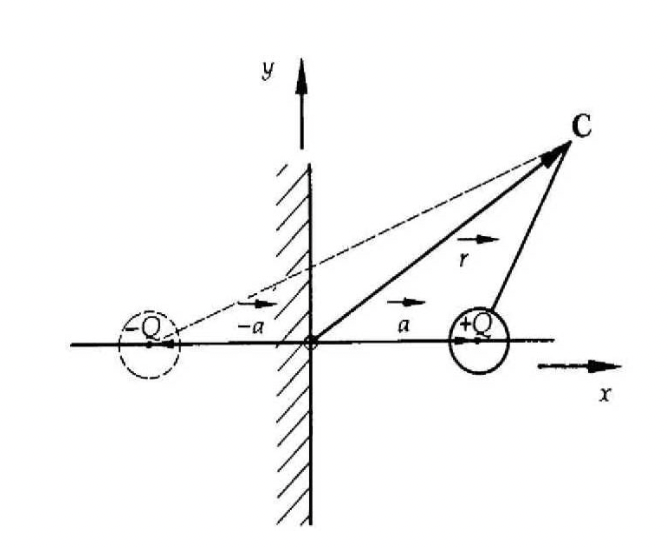
\includegraphics[scale=0.5]{media/graph9}
		\end{center}
		\caption{Схема методу електричних зображень.}
		\label{Picture_1}
	\end{figure}
	
	Розглянемо заряд $q$, що розташований на відстані $a$ від металевої поверхні під потенціалом землі (Рис. \ref{Picture_1}). Необхідно знайти поле в цьому напівпросторі. Це поле векторно складається з полів заряду $q$ та заряду, який індуковано на металевій поверхні. Однак поле індукованих зарядів еквівалентне полю уявного від'ємного заряду, який розташовано за поверхнею на відстані $a$. Дійсно, згідно з (Рис. \ref{Picture_1}) в довільній точці $C$ електричний потенціал, що обумовлюється зарядом $q$ та його уявним зображенням задається виразом:
	$$\varphi=q\bigg(\dfrac{1}{|\vec{r}-\vec{a}|}-\dfrac{1}{|\vec{r}-\vec{a}|}\bigg) \eqno(6)$$
	
	Згідно з (6) потенціал на поверхні дорівнює нулю і, таким чином, вираз (6) описує електричне поле в напівпросторі праворуч від металевої поверхні.
	
	
	
\newpage
	\begin{center}
		\section* {РОЗДІЛ 2. Теоретичні основи експерименту.}
	\end{center}
	\begin{figure}[h!]
		\begin{center}
			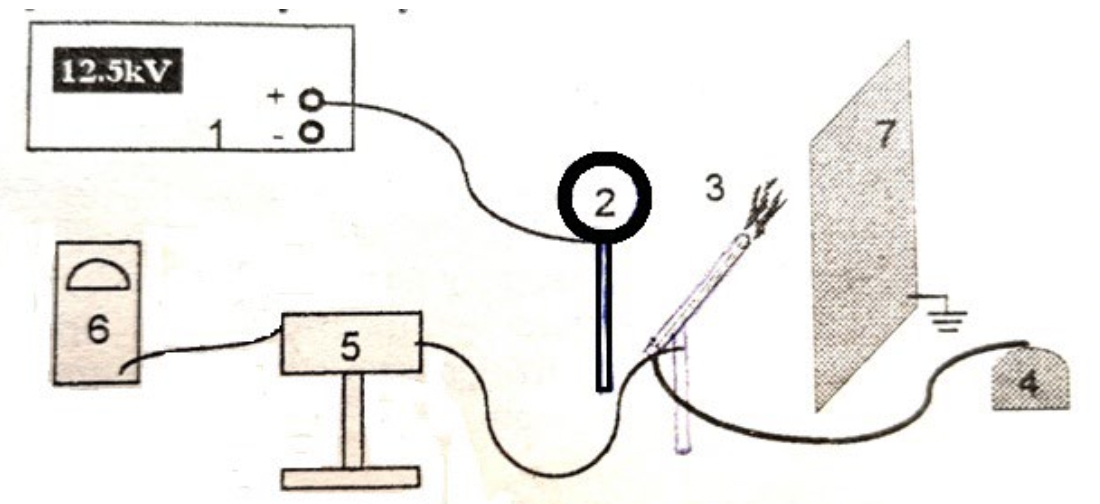
\includegraphics[scale=0.8]{media/graph10}
		\end{center}
		\caption{Схема дослідження потенціалів заряджених тіл та електростатичних полів.}
		\label{Picture_2}
	\end{figure}

	Високовольтне джерело напруги генерує напругу в межах 0 – 15 кВ, що встановлюється ступенями через 2.5 кВ. Максимальний струм короткого замикання (0.5 мА) та обмежена вихідна потужність (150 мДж) забезпечують безпечну роботу з джерелом напруги згідно з міжнародними вимогами VDЕ0411.
	
	Принцип дії вимірювача електричного поля такий. Електростатичне поле, що має бути виміряне, наводить індуктивні поверхневі заряди на двох електродах в вигляді зірки ізольованих один від одного і розташованих один проти одного. Поверхнева густина заряду прямо пропорційна інтенсивності електричного поля. Коліщатко в вигляді зірки, безперервно обертається перед одним з електродів і екранує його від поля, що вимірюється. Таким чином, генерується змінний струм індукованих зарядів який надалі підсилюється, спрямовується і вимірюється зовнішнім приладом. Електрометр може працювати в режимі виміру електричного поля та електричного потенціалу. Межа вимірюваного сигналу вста-новлюється за допомогою кнопок на верхній панелі. Подача газу з балону регулюється за допомогою ручки на редукторі.
\newpage

		\subsection{Хід експерименту}
	\begin{enumerate}
		\item  Зберіть схему експерименту по вивченню електростатичних полів згідно з (Рис. \ref{Picture_2}). Після перевірки схеми викладачем увімкніть прилади. Протестуйте електрометр 
		згідно з інструкцією по експлуатації. Встановіть напругу високовольтного джерела в межах 3 – 5 кВ.
		\item Встановіть в якості об’єкту, що досліджується, кульку. Відрегулюйте довжину полум’я зонда (зробіть його якомога менше).
		\item За допомогою координатної сітки зареєструйте ті положення кінчика зонду, які відповідають еквіпотенційним лініям. Для цього пересовуйте зонд в горизонтальній площині так, щоб значення поля залишалось незмінним. Всього бажано зафіксувати положення 10 – 12 еквіпотенційних ліній по 10 – 12 точок на кожну.
		\item Виміряйте розподіл потенціалу.
	\end{enumerate}
		\subsection{Завдання}
	\begin{enumerate}
		\item  За результатами п.3 зобразіть на площині $(X,\:Y)$ лінії рівного потенціалу, що утворює заряджена куля.
		\item За результатами п.3 побудуйте в графік залежності потенціалу електричного поля, що утворюється зарядженою кулею від відстані до центру кулі. Чому має дорівнювати тангенс кута нахилу цього графіку? Перевірте формулу (4.a).
		\item Зробіть висновки.
	\end{enumerate}\newpage
	\section{Роздiл 3. Експерементальнi данi.}
	\subsection{Графік залежності потенціалу електричного поля від відстані до центру кулі}
	\begin{figure*}[!h]
		\centering
			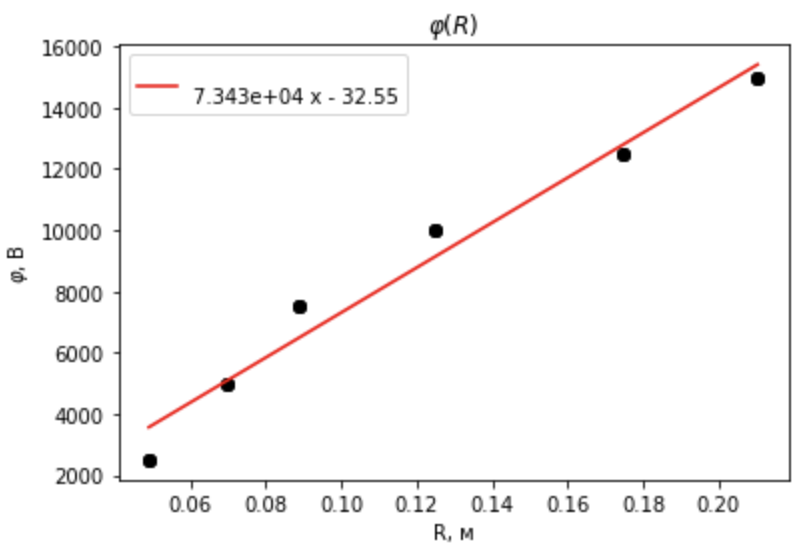
\includegraphics[height=80mm]{media/graph11aaa.png}
    		\caption{Апроксимована залежність потенціалу від відстані}
			\label{fig:8a}
    	\end{figure*}
	% Please add the following required packages to your document preamble:
% \usepackage{multirow}
\begin{table}[!h]
\label{table:table1}
	\begin{flushright}
		\caption{Дані}
	\end{flushright}
\begin{adjustwidth}{-1.25cm}{}
\begin{tabular}{|c|c|c|c|c|c|c|c|c|c|c|}
\hline
                   & $r$, м                 & $k,\>\dfrac{\textrm{Н}\cdot\textrm{м}^2}{\textrm{Кл}^2}$ & $\varphi$,  В          & $R$, м & $\langle R\rangle$, м  & $q$, Кл                     & $E, \textrm{Н}\cdot\textrm{Кл}$ & $R$(теор) , м          & $\Delta R$, м          & $\varepsilon R$,  \%   \\ \hline
\multirow{3}{*}{1} & \multirow{18}{*}{0.02} & \multirow{18}{*}{10000000000}                            & \multirow{3}{*}{2500}  & 0.05   & \multirow{3}{*}{0.049} & \multirow{3}{*}{0.00000001} & \multirow{18}{*}{14690.202}     & \multirow{3}{*}{0.058} & \multirow{3}{*}{0.001} & \multirow{3}{*}{1.178} \\ \cline{5-5}
                   &                        &                                                          &                        & 0.048  &                        &                             &                                 &                        &                        &                        \\ \cline{5-5}
                   &                        &                                                          &                        & 0.049  &                        &                             &                                 &                        &                        &                        \\ \cline{1-1} \cline{4-7} \cline{9-11} 
\multirow{3}{*}{2} &                        &                                                          & \multirow{3}{*}{5000}  & 0.07   & \multirow{3}{*}{0.07}  & \multirow{3}{*}{0.00000001} &                                 & \multirow{3}{*}{0.083} & \multirow{3}{*}{0.001} & \multirow{3}{*}{1.8}   \\ \cline{5-5}
                   &                        &                                                          &                        & 0.068  &                        &                             &                                 &                        &                        &                        \\ \cline{5-5}
                   &                        &                                                          &                        & 0.071  &                        &                             &                                 &                        &                        &                        \\ \cline{1-1} \cline{4-7} \cline{9-11} 
\multirow{3}{*}{3} &                        &                                                          & \multirow{3}{*}{7500}  & 0.088  & \multirow{3}{*}{0.089} & \multirow{3}{*}{0.00000001} &                                 & \multirow{3}{*}{0.101} & \multirow{3}{*}{0.001} & \multirow{3}{*}{1.178} \\ \cline{5-5}
                   &                        &                                                          &                        & 0.089  &                        &                             &                                 &                        &                        &                        \\ \cline{5-5}
                   &                        &                                                          &                        & 0.09   &                        &                             &                                 &                        &                        &                        \\ \cline{1-1} \cline{4-7} \cline{9-11} 
\multirow{3}{*}{4} &                        &                                                          & \multirow{3}{*}{10000} & 0.124  & \multirow{3}{*}{0.125} & \multirow{3}{*}{0.00000002} &                                 & \multirow{3}{*}{0.117} & \multirow{3}{*}{0.001} & \multirow{3}{*}{1.178} \\ \cline{5-5}
                   &                        &                                                          &                        & 0.125  &                        &                             &                                 &                        &                        &                        \\ \cline{5-5}
                   &                        &                                                          &                        & 0.126  &                        &                             &                                 &                        &                        &                        \\ \cline{1-1} \cline{4-7} \cline{9-11} 
\multirow{3}{*}{5} &                        &                                                          & \multirow{3}{*}{12500} & 0.175  & \multirow{3}{*}{0.175} & \multirow{3}{*}{0.00000002} &                                 & \multirow{3}{*}{0.13}  & \multirow{3}{*}{0.001} & \multirow{3}{*}{1.8}   \\ \cline{5-5}
                   &                        &                                                          &                        & 0.176  &                        &                             &                                 &                        &                        &                        \\ \cline{5-5}
                   &                        &                                                          &                        & 0.173  &                        &                             &                                 &                        &                        &                        \\ \cline{1-1} \cline{4-7} \cline{9-11} 
\multirow{3}{*}{6} &                        &                                                          & \multirow{3}{*}{15000} & 0.21   & \multirow{3}{*}{0.21}  & \multirow{3}{*}{0.00000003} &                                 & \multirow{3}{*}{0.143} & \multirow{3}{*}{0.001} & \multirow{3}{*}{1.8}   \\ \cline{5-5}
                   &                        &                                                          &                        & 0.209  &                        &                             &                                 &                        &                        &                        \\ \cline{5-5}
                   &                        &                                                          &                        & 0.212  &                        &                             &                                 &                        &                        &                        \\ \hline
\end{tabular}
\end{adjustwidth}
\end{table}\newpage
\subsection{Лінії рівного потенціалу}
	\begin{figure*}[!h]
		\centering
			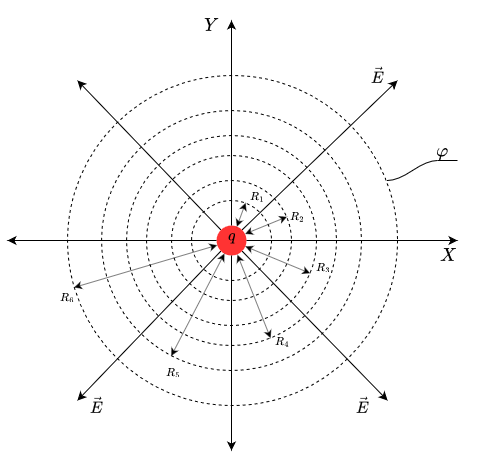
\includegraphics[height=90mm]{media/graph12.png}
    		\caption{Лінії рівного потенціалу на площині XY}
			\label{fig:8a}
    	\end{figure*}	
\subsection{Висновки}
За результатами обробки дослідних даних отримано залежність електричного потенціалу зарядженої кулі від відстані від центру кулі та напруженість поля, яке виникає при цьому, які дорівнюють, відповідно:
$$E=46519.068\textrm{ Н}\cdot\textrm{Кл}$$
Дослідні дані та результати обробки дослідних даних зведені до таблиці Таблиця 1. Як видно з графіку Рис. 3 залежність лінійна, що підтверджує 95\% досліджувані закони. Середня відносна похибка склала $\langle\varepsilon_R\rangle = 4.378\% \approx5\%$, за абсолютної 	похибки $\Delta R=0.001$ м. Причинами похибок 	могли стати такі 	фактори як 	вплив температури середовища на швидкість стікання заряду з кульки та 	похибка вимірювальних приладів.
	
	
	
	
	
	
	
	
	
	
	
	
	
	
	
	
	
	
	
	
	
	
	
	
	
	
	
	
	
	
	
	
	
	
	
	
	
	
	
	
	
	
	
	\end{justify}
\end{document}